
%% bare_conf.tex
%% V1.4b
%% 2015/08/26
%% by Michael Shell
%% See:
%% http://www.michaelshell.org/
%% for current contact information.
%%
%% This is a skeleton file demonstrating the use of IEEEtran.cls
%% (requires IEEEtran.cls version 1.8b or later) with an IEEE
%% conference paper.
%%
%% Support sites:
%% http://www.michaelshell.org/tex/ieeetran/
%% http://www.ctan.org/pkg/ieeetran
%% and
%% http://www.ieee.org/

%%*************************************************************************
%% Legal Notice:
%% This code is offered as-is without any warranty either expressed or
%% implied; without even the implied warranty of MERCHANTABILITY or
%% FITNESS FOR A PARTICULAR PURPOSE! 
%% User assumes all risk.
%% In no event shall the IEEE or any contributor to this code be liable for
%% any damages or losses, including, but not limited to, incidental,
%% consequential, or any other damages, resulting from the use or misuse
%% of any information contained here.
%%
%% All comments are the opinions of their respective authors and are not
%% necessarily endorsed by the IEEE.
%%
%% This work is distributed under the LaTeX Project Public License (LPPL)
%% ( http://www.latex-project.org/ ) version 1.3, and may be freely used,
%% distributed and modified. A copy of the LPPL, version 1.3, is included
%% in the base LaTeX documentation of all distributions of LaTeX released
%% 2003/12/01 or later.
%% Retain all contribution notices and credits.
%% ** Modified files should be clearly indicated as such, including  **
%% ** renaming them and changing author support contact information. **
%%*************************************************************************


% *** Authors should verify (and, if needed, correct) their LaTeX system  ***
% *** with the testflow diagnostic prior to trusting their LaTeX platform ***
% *** with production work. The IEEE's font choices and paper sizes can   ***
% *** trigger bugs that do not appear when using other class files.       ***                          ***
% The testflow support page is at:
% http://www.michaelshell.org/tex/testflow/



\documentclass[conference]{IEEEtran}
\usepackage{graphicx}
\graphicspath{{D:\\Masters\\Spring\ 2016\\AI\\N-Queens\ project}}
\DeclareGraphicsExtensions{.png}

\usepackage{textcomp}
% Some Computer Society conferences also require the compsoc mode option,
% but others use the standard conference format.
%
% If IEEEtran.cls has not been installed into the LaTeX system files,
% manually specify the path to it like:
% \documentclass[conference]{../sty/IEEEtran}





% Some very useful LaTeX packages include:
% (uncomment the ones you want to load)


% *** MISC UTILITY PACKAGES ***
%
%\usepackage{ifpdf}
% Heiko Oberdiek's ifpdf.sty is very useful if you need conditional
% compilation based on whether the output is pdf or dvi.
% usage:
% \ifpdf
%   % pdf code
% \else
%   % dvi code
% \fi
% The latest version of ifpdf.sty can be obtained from:
% http://www.ctan.org/pkg/ifpdf
% Also, note that IEEEtran.cls V1.7 and later provides a builtin
% \ifCLASSINFOpdf conditional that works the same way.
% When switching from latex to pdflatex and vice-versa, the compiler may
% have to be run twice to clear warning/error messages.






% *** CITATION PACKAGES ***
%
%\usepackage{cite}
% cite.sty was written by Donald Arseneau
% V1.6 and later of IEEEtran pre-defines the format of the cite.sty package
% \cite{} output to follow that of the IEEE. Loading the cite package will
% result in citation numbers being automatically sorted and properly
% "compressed/ranged". e.g., [1], [9], [2], [7], [5], [6] without using
% cite.sty will become [1], [2], [5]--[7], [9] using cite.sty. cite.sty's
% \cite will automatically add leading space, if needed. Use cite.sty's
% noadjust option (cite.sty V3.8 and later) if you want to turn this off
% such as if a citation ever needs to be enclosed in parenthesis.
% cite.sty is already installed on most LaTeX systems. Be sure and use
% version 5.0 (2009-03-20) and later if using hyperref.sty.
% The latest version can be obtained at:
% http://www.ctan.org/pkg/cite
% The documentation is contained in the cite.sty file itself.






% *** GRAPHICS RELATED PACKAGES ***
%
\ifCLASSINFOpdf
  % \usepackage[pdftex]{graphicx}
  % declare the path(s) where your graphic files are
  % \graphicspath{{../pdf/}{../jpeg/}}
  % and their extensions so you won't have to specify these with
  % every instance of \includegraphics
  % \DeclareGraphicsExtensions{.pdf,.jpeg,.png}
\else
  % or other class option (dvipsone, dvipdf, if not using dvips). graphicx
  % will default to the driver specified in the system graphics.cfg if no
  % driver is specified.
  % \usepackage[dvips]{graphicx}
  % declare the path(s) where your graphic files are
  % \graphicspath{{../eps/}}
  % and their extensions so you won't have to specify these with
  % every instance of \includegraphics
  % \DeclareGraphicsExtensions{.eps}
\fi
% graphicx was written by David Carlisle and Sebastian Rahtz. It is
% required if you want graphics, photos, etc. graphicx.sty is already
% installed on most LaTeX systems. The latest version and documentation
% can be obtained at: 
% http://www.ctan.org/pkg/graphicx
% Another good source of documentation is "Using Imported Graphics in
% LaTeX2e" by Keith Reckdahl which can be found at:
% http://www.ctan.org/pkg/epslatex
%
% latex, and pdflatex in dvi mode, support graphics in encapsulated
% postscript (.eps) format. pdflatex in pdf mode supports graphics
% in .pdf, .jpeg, .png and .mps (metapost) formats. Users should ensure
% that all non-photo figures use a vector format (.eps, .pdf, .mps) and
% not a bitmapped formats (.jpeg, .png). The IEEE frowns on bitmapped formats
% which can result in "jaggedy"/blurry rendering of lines and letters as
% well as large increases in file sizes.
%
% You can find documentation about the pdfTeX application at:
% http://www.tug.org/applications/pdftex





% *** MATH PACKAGES ***
%
%\usepackage{amsmath}
% A popular package from the American Mathematical Society that provides
% many useful and powerful commands for dealing with mathematics.
%
% Note that the amsmath package sets \interdisplaylinepenalty to 10000
% thus preventing page breaks from occurring within multiline equations. Use:
%\interdisplaylinepenalty=2500
% after loading amsmath to restore such page breaks as IEEEtran.cls normally
% does. amsmath.sty is already installed on most LaTeX systems. The latest
% version and documentation can be obtained at:
% http://www.ctan.org/pkg/amsmath





% *** SPECIALIZED LIST PACKAGES ***
%
%\usepackage{algorithmic}
% algorithmic.sty was written by Peter Williams and Rogerio Brito.
% This package provides an algorithmic environment fo describing algorithms.
% You can use the algorithmic environment in-text or within a figure
% environment to provide for a floating algorithm. Do NOT use the algorithm
% floating environment provided by algorithm.sty (by the same authors) or
% algorithm2e.sty (by Christophe Fiorio) as the IEEE does not use dedicated
% algorithm float types and packages that provide these will not provide
% correct IEEE style captions. The latest version and documentation of
% algorithmic.sty can be obtained at:
% http://www.ctan.org/pkg/algorithms
% Also of interest may be the (relatively newer and more customizable)
% algorithmicx.sty package by Szasz Janos:
% http://www.ctan.org/pkg/algorithmicx




% *** ALIGNMENT PACKAGES ***
%
%\usepackage{array}
% Frank Mittelbach's and David Carlisle's array.sty patches and improves
% the standard LaTeX2e array and tabular environments to provide better
% appearance and additional user controls. As the default LaTeX2e table
% generation code is lacking to the point of almost being broken with
% respect to the quality of the end results, all users are strongly
% advised to use an enhanced (at the very least that provided by array.sty)
% set of table tools. array.sty is already installed on most systems. The
% latest version and documentation can be obtained at:
% http://www.ctan.org/pkg/array


% IEEEtran contains the IEEEeqnarray family of commands that can be used to
% generate multiline equations as well as matrices, tables, etc., of high
% quality.




% *** SUBFIGURE PACKAGES ***
\ifCLASSOPTIONcompsoc
  \usepackage[caption=false,font=normalsize,labelfont=sf,textfont=sf]{subfig}
\else
  \usepackage[caption=false,font=footnotesize]{subfig}
\fi
% subfig.sty, written by Steven Douglas Cochran, is the modern replacement
% for subfigure.sty, the latter of which is no longer maintained and is
% incompatible with some LaTeX packages including fixltx2e. However,
% subfig.sty requires and automatically loads Axel Sommerfeldt's caption.sty
% which will override IEEEtran.cls' handling of captions and this will result
% in non-IEEE style figure/table captions. To prevent this problem, be sure
% and invoke subfig.sty's "caption=false" package option (available since
% subfig.sty version 1.3, 2005/06/28) as this is will preserve IEEEtran.cls
% handling of captions.
% Note that the Computer Society format requires a larger sans serif font
% than the serif footnote size font used in traditional IEEE formatting
% and thus the need to invoke different subfig.sty package options depending
% on whether compsoc mode has been enabled.
%
% The latest version and documentation of subfig.sty can be obtained at:
% http://www.ctan.org/pkg/subfig




% *** FLOAT PACKAGES ***
%
%\usepackage{fixltx2e}
% fixltx2e, the successor to the earlier fix2col.sty, was written by
% Frank Mittelbach and David Carlisle. This package corrects a few problems
% in the LaTeX2e kernel, the most notable of which is that in current
% LaTeX2e releases, the ordering of single and double column floats is not
% guaranteed to be preserved. Thus, an unpatched LaTeX2e can allow a
% single column figure to be placed prior to an earlier double column
% figure.
% Be aware that LaTeX2e kernels dated 2015 and later have fixltx2e.sty's
% corrections already built into the system in which case a warning will
% be issued if an attempt is made to load fixltx2e.sty as it is no longer
% needed.
% The latest version and documentation can be found at:
% http://www.ctan.org/pkg/fixltx2e


%\usepackage{stfloats}
% stfloats.sty was written by Sigitas Tolusis. This package gives LaTeX2e
% the ability to do double column floats at the bottom of the page as well
% as the top. (e.g., "\begin{figure*}[!b]" is not normally possible in
% LaTeX2e). It also provides a command:
%\fnbelowfloat
% to enable the placement of footnotes below bottom floats (the standard
% LaTeX2e kernel puts them above bottom floats). This is an invasive package
% which rewrites many portions of the LaTeX2e float routines. It may not work
% with other packages that modify the LaTeX2e float routines. The latest
% version and documentation can be obtained at:
% http://www.ctan.org/pkg/stfloats
% Do not use the stfloats baselinefloat ability as the IEEE does not allow
% \baselineskip to stretch. Authors submitting work to the IEEE should note
% that the IEEE rarely uses double column equations and that authors should try
% to avoid such use. Do not be tempted to use the cuted.sty or midfloat.sty
% packages (also by Sigitas Tolusis) as the IEEE does not format its papers in
% such ways.
% Do not attempt to use stfloats with fixltx2e as they are incompatible.
% Instead, use Morten Hogholm'a dblfloatfix which combines the features
% of both fixltx2e and stfloats:
%
% \usepackage{dblfloatfix}
% The latest version can be found at:
% http://www.ctan.org/pkg/dblfloatfix




% *** PDF, URL AND HYPERLINK PACKAGES ***
%
%\usepackage{url}
% url.sty was written by Donald Arseneau. It provides better support for
% handling and breaking URLs. url.sty is already installed on most LaTeX
% systems. The latest version and documentation can be obtained at:
% http://www.ctan.org/pkg/url
% Basically, \url{my_url_here}.




% *** Do not adjust lengths that control margins, column widths, etc. ***
% *** Do not use packages that alter fonts (such as pslatex).         ***
% There should be no need to do such things with IEEEtran.cls V1.6 and later.
% (Unless specifically asked to do so by the journal or conference you plan
% to submit to, of course. )


% correct bad hyphenation here
\hyphenation{op-tical net-works semi-conduc-tor}


\begin{document}
%
% paper title
% Titles are generally capitalized except for words such as a, an, and, as,
% at, but, by, for, in, nor, of, on, or, the, to and up, which are usually
% not capitalized unless they are the first or last word of the title.
% Linebreaks \\ can be used within to get better formatting as desired.
% Do not put math or special symbols in the title.
\title{Experimental comparison of AI algorithms to solve N-Queens problem }


% author names and affiliations
% use a multiple column layout for up to three different
% affiliations
\author{\IEEEauthorblockN{Ashwini Karappa}
\IEEEauthorblockA{Masters Student, Department of Computer Science.\\
University of Texas at Dallas\\
Richardson, Texas 75080, USA.\\
Email: axk142031@utdallas.edu}}


% conference papers do not typically use \thanks and this command
% is locked out in conference mode. If really needed, such as for
% the acknowledgment of grants, issue a \IEEEoverridecommandlockouts
% after \documentclass

% for over three affiliations, or if they all won't fit within the width
% of the page, use this alternative format:
% 
%\author{\IEEEauthorblockN{Michael Shell\IEEEauthorrefmark{1},
%Homer Simpson\IEEEauthorrefmark{2},
%James Kirk\IEEEauthorrefmark{3}, 
%Montgomery Scott\IEEEauthorrefmark{3} and
%Eldon Tyrell\IEEEauthorrefmark{4}}
%\IEEEauthorblockA{\IEEEauthorrefmark{1}School of Electrical and Computer Engineering\\
%Georgia Institute of Technology,
%Atlanta, Georgia 30332--0250\\ Email: see http://www.michaelshell.org/contact.html}
%\IEEEauthorblockA{\IEEEauthorrefmark{2}Twentieth Century Fox, Springfield, USA\\
%Email: homer@thesimpsons.com}
%\IEEEauthorblockA{\IEEEauthorrefmark{3}Starfleet Academy, San Francisco, California 96678-2391\\
%Telephone: (800) 555--1212, Fax: (888) 555--1212}
%\IEEEauthorblockA{\IEEEauthorrefmark{4}Tyrell Inc., 123 Replicant Street, Los Angeles, California 90210--4321}}




% use for special paper notices
%\IEEEspecialpapernotice{(Invited Paper)}




% make the title area
\maketitle

% As a general rule, do not put math, special symbols or citations
% in the abstract
\begin{abstract}
This report discusses different techniques known for solving constraint satisfaction problems. I implemented few of these techniques which are namely backtracking, forward checking, variable ordering using minimum remaining values and minimum conflicts for solving N-Queens puzzle. N-Queens problem has some practical applications such as in traffic control, deadlock prevention, statistics, and parallel memory storage schemes. It is often used as an example of constraint satisfaction problem. I also present an experimental comparison of the techniques that I implemented for solving this puzzle. 
\\
\\\smallskip
\textit{Keywords---}
Constraint satisfaction problem, N-Queens, Backtracking, Forward checking,Variable ordering and Value ordering, Minimum Conflicts

\end{abstract}

% no keywords



% For peer review papers, you can put extra information on the cover
% page as needed:
% \ifCLASSOPTIONpeerreview
% \begin{center} \bfseries EDICS Category: 3-BBND \end{center}
% \fi
%
% For peerreview papers, this IEEEtran command inserts a page break and
% creates the second title. It will be ignored for other modes.
\IEEEpeerreviewmaketitle



\section{Introduction and Background [1,2]}

We come across various puzzles based on chessboards such as counting the number of squares, counting the number of rectangles and finding the best moves. The n-queens problem is one of the chess puzzles. This problem was originally known as the 8-Queens problem. It has been of interest for many mathematicians. It was generalized to N-Queens for N X N boards in 1850 by Franz Nauck. According to the chess rules, queens can attack by moving forward or backward in the same row, the same column or the same diagonal. N-Queens puzzle asks, 'How to place N queens on N X N chess board, such that no two of them can attack each other?'. Figure 1, shows an example of 4-Queens problem. Part a), in figure 1, shows the wrong placement of queens, because the queens in second row and third row can attack each other since they lie on the same diagonal. Part b), in figure 1, shows the correct placement of 4 queens where no two queens can attack each other. 
\par N-Queens puzzle has many practical applications like parallel memory storage schemes, VLSI testing, traffic control and deadlock prevention. This problem is an example of  backtracking algorithms, permutation generation, the divide and conquer paradigm, program development methodology, constraint satisfaction problems, integer programming, and specification. Thus, with the rapid development of computer science, N-Queens problem has gained a lot of attention and solving it with optimal techniques has gained importance.
\par This report initially explains different AI techniques people experimented on to solve this puzzle in related work. Further, I explain constraint satisfaction problem solving techniques namely: backtracking, forward checking, forward checking with MRV and minimum conflicts that I implemented for solving N-Queens puzzle. I also present the experimental results of these algorithms and my key observations. Finally, I conclude the paper.

\begin{figure}%
    \centering
    \subfloat[Wrong placement]{{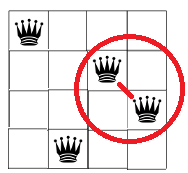
\includegraphics[width=2.25 cm]{4QueensWrongSolution.png} }}%
    \label{Figure6}
    \qquad
    \subfloat[Correct placement]{{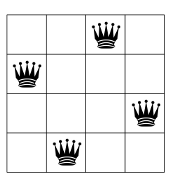
\includegraphics[width=2cm]{4QueensCorrectSolution.png} }}%
    \\
    \centering
 
    \label{Figure7}
\label{figure1}
\caption{Example of 4 Queens puzzle}
\end{figure}


 
% no \IEEEPARstart
% You must have at least 2 lines in the paragraph with the drop letter
% (should never be an issue)




\section{Related work}
Previously,  lots  of  work  is  done  on  N-Queens  problem. This problem can be solved using different techniques. Kuruvilla Mathew and Mujahid Tabassum in [3], compared the performances of search strategies namely: Breadth  First  Search,  Depth First Search, A* Search, Greedy Best First Search and the  Hill  Climbing  Search to solve 8 queens problem. They concluded that A* is the best strategy amongst the others listed and it achieves convergence faster, at cheaper cost, and therefore they also suggest that A* is  best  suited  for  solving  issues  of  this  nature and also  has  the possibilities  to  be  applied  towards  issues  of  growing dimensionalities.	 K.  D. Crawford  in  [4],  applied  Genetic  Algorithm  and  have discussed  two  ways  to  solve  n-Queen  problem. Marko Božiković, Marin Golub, Leo Budin in [5], show how genetic  algorithms can  be  used  to  solve  n-Queen  problem. In this paper, they have also shared their experimental results for several large values of n and their conclusions for NP problems with genetic algorithms.

\section{Constraint satisfaction problems}

Although, there are many ways of solving N-queens puzzle, it mainly falls under and is well known as  constraint satisfaction  problem. Constraint satisfaction problems are basically the problems in which there is a set of variables and a set of values. Each variable is to be assigned a value, such that, it satisfies all the constraints for the problem. N-Queens puzzle, thus, is a constraint satisfaction problem, where queens are to be placed such that no two can attack each other.

\section{Constraint Satisfaction problem solving techniques implemented[6,7]}

 
\textbf{Soling N-Queens Problem}
\par In N-Queens problem, no two queens should be on the same row or the same column or the same diagonal. I have implemented Backtracking, Forward checking, Forward checking with minimum remaining values and Minimum conflicts techniques for solving N-Queens puzzle. In the following section, I have explained in brief these techniques and illustrated them with 4 Queens example. Backtracking and forward checking examples are taken from [7]. I have created a similar example for forward checking with minimum remaining values and the example for minimum conflicts is taken from the book [6]. In the example figures, queens are placed column wise. There are 'N' columns and 'N' rows in a 'N x N' chess board. First Column has 'N' cells, because of 'N' rows, Second column also has 'N' cells and so on. These techniques, place queens column wise. In each column, one queen will be placed on any of the 'N' cells by selecting the row such that, it satisfies the constraints for N-Queens puzzle. For figures 2, 3, and 4 we have 4 x 4 chess boards. And red dot denotes the queen and cross mark denotes the places where queens cannot be placed. In figure 5, we have 8 x 8 chess board for minimum conflicts.

\subsection{Backtracking}
 Backtracking is a simple depth first search approach. It starts initially with any variable, assigns a value from the domain of values and then goes deeper into the tree to assign values to other variables. Later on, at some level, if it finds out that there are no values left for a variable, it backtracks and assigns different value to the parent variables. Figure 2, shows an example to understand backtracking approach for solving 4-queens problem.
 
 \textbf{Explaining the example- }

1. First queen is placed in the first column and the first available row. Initially for the first queen it is first column and first row, then it goes down into the search tree and check assignments for other queens.
\par 2. Second queen is placed in the second column, initially it checks whether placing second queen in the second column and first row is possible, then the algorithm understands that this is not the valid place. Thus, it goes to the second row, again it understands that this is not the valid place, then it places the queen in the third row.
\par 3. It again goes down deeper into the tree and does the same thing for other queens.
\par 4. But if for some queen, it does not find a cell to place the queen, it backtracks on the previous level and checks other places for the previously placed queens.
\par 5. This algorithm will go on until the last queen is placed.

\begin{figure}
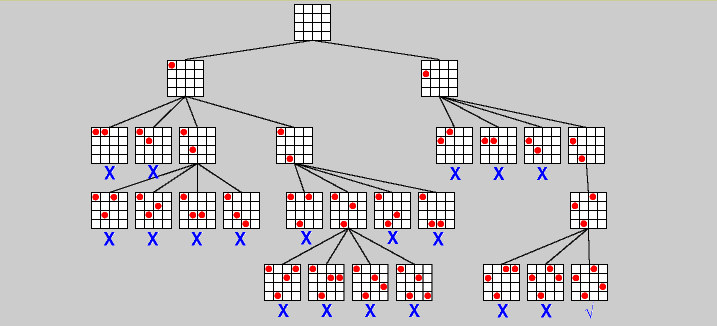
\includegraphics[scale=0.5]{Backtracking.png}
\caption{Backtracking approach}
\label{Figure2}
\end{figure}


\subsection{Forward Checking}

Generally, in most of the constraint satisfaction problems, as soon as any variable is assigned a value, this value is no longer valid for some of the other variables. Forward checking is the technique which is nothing but backtracking, but it also saves the effect of variables assigned with values in the previous step and grows the search tree only for the assignments which are valid.

 \textbf{Explaining the example- }
\\ Figure 3, shows an example of forward checking approach for solving 4 Queens problem. In this example, we can see that, once a queen is placed, all the cells in its row, column and diagonals where other queens cannot be placed are marked with a cross. So, when the search tree goes deeper, it knows which cells cannot be considered for the placement of the current queen. Thus, the search tree that grows is smaller as compared to the backtracking. 

\begin{figure}
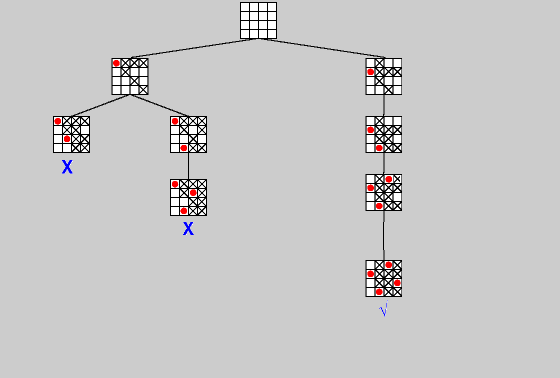
\includegraphics[scale=0.65]{ForwardChecking.png}
\caption{Forward Checking approach}
\label{Figure3}
\end{figure}

In my implementation of this algorithm, for every recursive call, I maintain an old and a new boolean N X N chessboard. As soon as I enter into the recursive call, I make a new chessboard from the old chessboard. I update the new one with false values for the cells which are no longer valid for other queens because of the place assigned for the current queen. When algorithm backtracks, it has the old chessboard, which it can use for checking other places for previously assigned queens.

\subsection{Variable Ordering and Value Ordering}

Backtracking and Forward checking both these techniques do not use any special order for assigning values to the variables. Variable ordering technique is based on an intuitive idea of giving preference to the variable which is left with the fewest possible “legal” values. This is also called as "Minimum Remaining Values", (MRV) heuristic. Value ordering heuristic known as "Least Constraining Values", (LCV) heuristics,  prefers the values that rules out the fewest choices for the neighboring variables in the constraint graph.

We can apply MRV and LCV heuristics, both as a combination or individually on backtracking as well as forward checking. For experimental analysis, I have implemented MRV heuristic for forward checking. Figure  4 shows an example for the same. \\

\textbf {Explaining the example- }

In this example, initially every queen has minimum remaining values (MRV) equal to 4, since none of the queens have been placed. As MRV is same for all the queens, algorithm selects any queen randomly for the assignment. In the example shown, randomly 4th queen is selected for placement. Then, it marks the the cells with a cross which are ruled out for other queens. Similarly it repeats the process when going down further for other queens. If MRV becomes zero for any queen, algorithm backtracks as shown on the left branch of the tree. On the right branch of the tree, it can be seen on 3rd level, that MRV for queen 1 = 2, and queen 2 = 1, thus on the next step, algorithm first selects queen 2 for the placement.
\\Algorithm terminates when all the four queens are placed with a valid placement. 


\begin{figure}
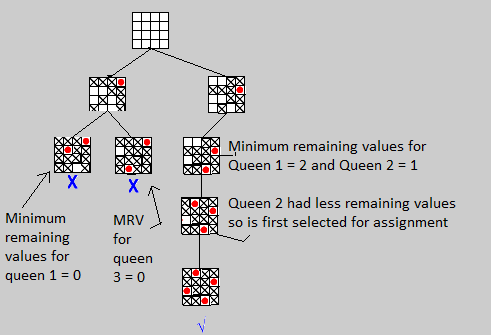
\includegraphics[scale=0.65]{ForwardCheckingWithMRV.png}
\caption{Forward checking with minimum remaining values approach}
\label{Figure4}
\end{figure}


In my implementation of this algorithm, I am maintaining a minimum priority queue, which after every  assignment of any queen, gives me the queen with the minimum remaining legal values for placement. I select this queen and assign a place to it and repeat the process of adding remaining queens to the queue with updated remaining values. Also, when the algorithm backtracks, I again update the priority queue for queens with minimum remaining values.

\subsection{Minimum Conflicts}

In this technique, a complete random assignment is taken for all the variables. Then the variables that are under conflicts, i.e, the ones which violates the constrains are computed. Randomly any variable under conflict is reassigned to some other value by computing the value which will have least number of conflicts. Again conflicts for all the variables are computed, and the same process of reassigning the values to the variables in conflicts is repeated until there are no conflicts.

Figure 5, shows an example for minimum conflicts [6]. 
\begin{figure}
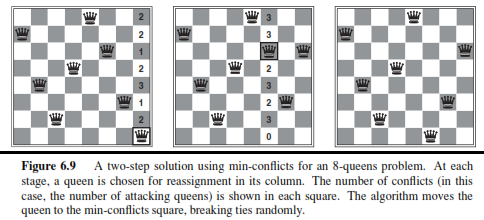
\includegraphics[scale=0.65]{MinimumConflicts.png}
\caption{Minimum Conflicts approach}
\label{Figure5}
\end{figure}

In my implementation of this algorithm, I am maintaining a max priority queue which after every complete random assignment of the problem, gives me the queen with the maximum number of conflicts and I select this queen for reassignment to the values which will have least number of conflicts. Again, conflicts are computed for all the queens and the process of reassigning the maximum priority queens (those with max number of conflicts) repeats until there are not conflicts.


% An example of a floating figure using the graphicx package.
% Note that \label must occur AFTER (or within) \caption.
% For figures, \caption should occur after the \includegraphics.
% Note that IEEEtran v1.7 and later has special internal code that
% is designed to preserve the operation of \label within \caption
% even when the captionsoff option is in effect. However, because
% of issues like this, it may be the safest practice to put all your
% \label just after \caption rather than within \caption{}.
%
% Reminder: the "draftcls" or "draftclsnofoot", not "draft", class
% option should be used if it is desired that the figures are to be
% displayed while in draft mode.
%
%\begin{figure}[!t]
%\centering
%\includegraphics[width=2.5in]{myfigure}
% where an .eps filename suffix will be assumed under latex, 
% and a .pdf suffix will be assumed for pdflatex; or what has been declared
% via \DeclareGraphicsExtensions.
%\caption{Simulation results for the network.}
%\label{fig_sim}
%\end{figure}

% Note that the IEEE typically puts floats only at the top, even when this
% results in a large percentage of a column being occupied by floats.


% An example of a double column floating figure using two subfigures.
% (The subfig.sty package must be loaded for this to work.)
% The subfigure \label commands are set within each subfloat command,
% and the \label for the overall figure must come after \caption.
% \hfil is used as a separator to get equal spacing.
% Watch out that the combined width of all the subfigures on a 
% line do not exceed the text width or a line break will occur.
%
%\begin{figure*}[!t]
%\centering
%\subfloat[Case I]{\includegraphics[width=2.5in]{box}%
%\label{fig_first_case}}
%\hfil
%\subfloat[Case II]{\includegraphics[width=2.5in]{box}%
%\label{fig_second_case}}
%\caption{Simulation results for the network.}
%\label{fig_sim}
%\end{figure*}
%
% Note that often IEEE papers with subfigures do not employ subfigure
% captions (using the optional argument to \subfloat[]), but instead will
% reference/describe all of them (a), (b), etc., within the main caption.
% Be aware that for subfig.sty to generate the (a), (b), etc., subfigure
% labels, the optional argument to \subfloat must be present. If a
% subcaption is not desired, just leave its contents blank,
% e.g., \subfloat[].


% An example of a floating table. Note that, for IEEE style tables, the
% \caption command should come BEFORE the table and, given that table
% captions serve much like titles, are usually capitalized except for words
% such as a, an, and, as, at, but, by, for, in, nor, of, on, or, the, to
% and up, which are usually not capitalized unless they are the first or
% last word of the caption. Table text will default to \footnotesize as
% the IEEE normally uses this smaller font for tables.
% The \label must come after \caption as always.
%
%\begin{table}[!t]
%% increase table row spacing, adjust to taste
%\renewcommand{\arraystretch}{1.3}
% if using array.sty, it might be a good idea to tweak the value of
% \extrarowheight as needed to properly center the text within the cells
%\caption{An Example of a Table}
%\label{table_example}
%\centering
%% Some packages, such as MDW tools, offer better commands for making tables
%% than the plain LaTeX2e tabular which is used here.
%\begin{tabular}{|c||c|}
%\hline
%One & Two\\
%\hline
%Three & Four\\
%\hline
%\end{tabular}
%\end{table}


% Note that the IEEE does not put floats in the very first column
% - or typically anywhere on the first page for that matter. Also,
% in-text middle ("here") positioning is typically not used, but it
% is allowed and encouraged for Computer Society conferences (but
% not Computer Society journals). Most IEEE journals/conferences use
% top floats exclusively. 
% Note that, LaTeX2e, unlike IEEE journals/conferences, places
% footnotes above bottom floats. This can be corrected via the
% \fnbelowfloat command of the stfloats package.




% conference papers do not normally have an appendix


% use section* for acknowledgment
%\section*{Acknowledgment}


%The authors would like to thank...





% trigger a \newpage just before the given reference
% number - used to balance the columns on the last page
% adjust value as needed - may need to be readjusted if
% the document is modified later
%\IEEEtriggeratref{8}
% The "triggered" command can be changed if desired:
%\IEEEtriggercmd{\enlargethispage{-5in}}

% references section

% can use a bibliography generated by BibTeX as a .bbl file
% BibTeX documentation can be easily obtained at:
% http://mirror.ctan.org/biblio/bibtex/contrib/doc/
% The IEEEtran BibTeX style support page is at:
% http://www.michaelshell.org/tex/ieeetran/bibtex/
%\bibliographystyle{IEEEtran}
% argument is your BibTeX string definitions and bibliography database(s)
%\bibliography{IEEEabrv,../bib/paper}
%
% <OR> manually copy in the resultant .bbl file
% set second argument of \begin to the number of references
% (used to reserve space for the reference number labels box)

\section{Project Application Information}

I have developed a project for solving N-Queens problem with the help of four techniques discussed above.
Figure 7, shows a snap shot of my application. On left side, there is a dropdown to select the algorithm, and a dropdown to select the 'N' value and when you click on solve, you will see all the solutions on the right hand side. And if you select any particular solution from the dropdown of solutions on right side, you will see the chessboard with N-Queens placed for that solution.

\par In the dropdown on the left side for inputs, if you select the COMPARE\_NUMBER\_OF\_NODES\_COMPUTED, you will see a comparison graph for the number of nodes computed in the search tree in order to get the first solution each, using all the four techiques. Example is shown in figure 6.

\par  In the dropdown, if you select the COMPARE\_TIME\_REQUIRED, you will see a comparison graph for the the time required in order to get first solution each, using all the four techiques.


\begin{figure}
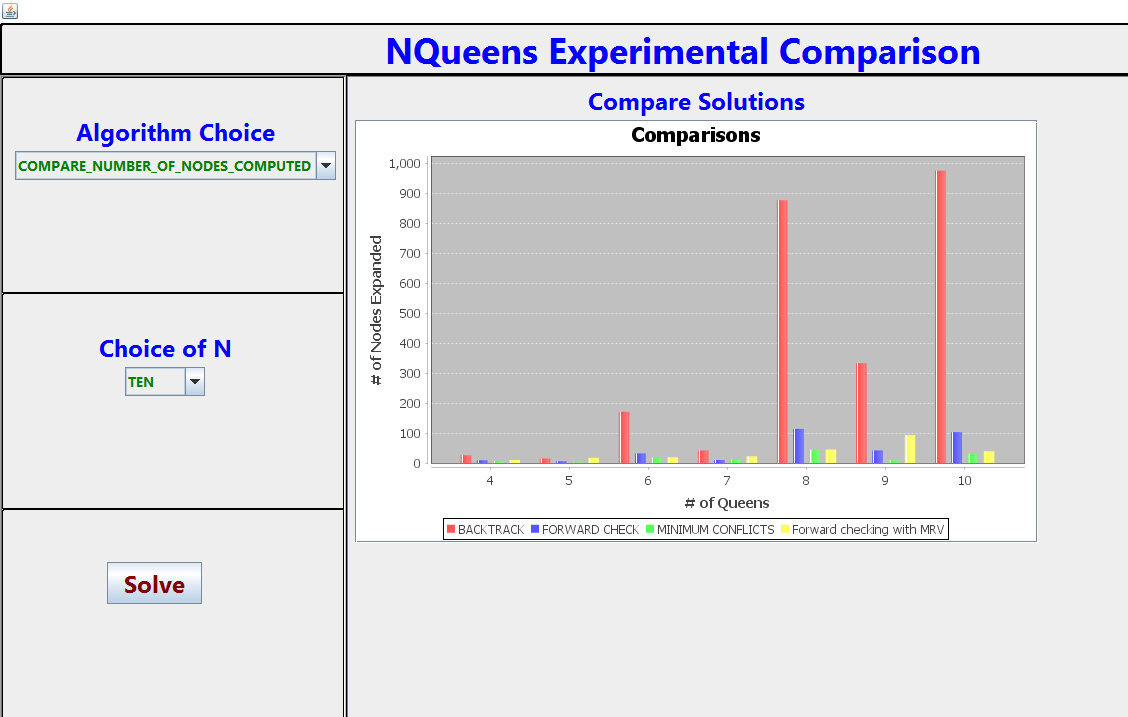
\includegraphics[scale=0.27]{N10nodesComputedComparison.png}
\caption{Application image for showing comparison}
\label{Figure9}
\end{figure}


\begin{figure}
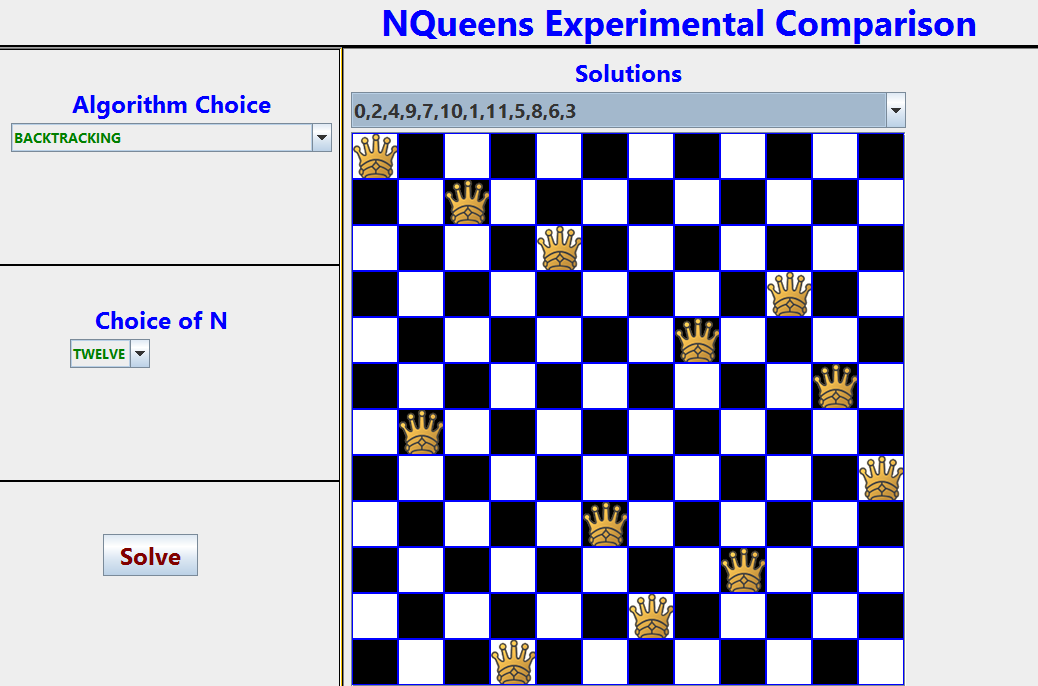
\includegraphics[scale=0.3]{BacktrackingNqueensSoln.png}
\caption{Application image for showing NQueens solutions}
\label{Figure9}
\end{figure}

\section{Experimental Results}

I have analyzed the performance of the mentioned four algorithms based on the number of nodes computed and time required to compute the solutions. Backtracking and forward checking techniques generate a search tree, where nodes represent the states of the chessboard. At each level a new queen is placed and on the same level sibling nodes denote different cells checked for placing the queen.
\par \textbf{Performance based on nodes computed}
\par Backtracking checks all the places for every queen. That is, if there are 'd' domain values and 'N' variables then the search tree generated will be of n!d leaves, which is very huge. Thus the number of nodes computed for backtracking is the highest.
\par Forward checking, rules out the values for next queen to be placed based on the previous queens assignment. Thus, the number of nodes computed in this case is less as compared to the backtracking approach. But, when we compare it with forward checking with MRV, nodes computed would be less or more. Reason being, Forward checking with MRV heuristic, randomly selects the queens, when every queen has the same minimum remaining values. Thus, if the queen selected randomly, gives a node which is closer to the solution, then forward checking with MRV heuristics will compute lesser nodes as compared to the forward checking.
\par Minimum Conflicts starts with a random complete assignment. Thus, it eliminates the nodes that are computed for initial queen placements. This improves the performance to a great extent. I found out that even for N=1000, this algorithm solves N-Queens puzzle on an average just within 350 steps. Thus, this approach performes the best as compared to the other three techniques.
\\ Figure 8, shows the analysis of nodes computed for N = 4 to N = 15.



\par \textbf{Performance based on time required}

As analyzed for N=4 till N=15, Backtracking requires very less time as compared to forward checking as well as forward checking with MRV. Reason for this behavior is because, backtracking requires very less computations as compared to forward checking and and forward checking with MRV though its search tree is larger. Forward checking and forward checking with MRV have to compute unsafe places for next all the queens based on the previous queen's assignment which eats up more time. Minimum conflicts is as compared to the other three techniques, is very fast, since it eliminates initial queen placements and starts directly with a random complete assignment.

\begin{figure}
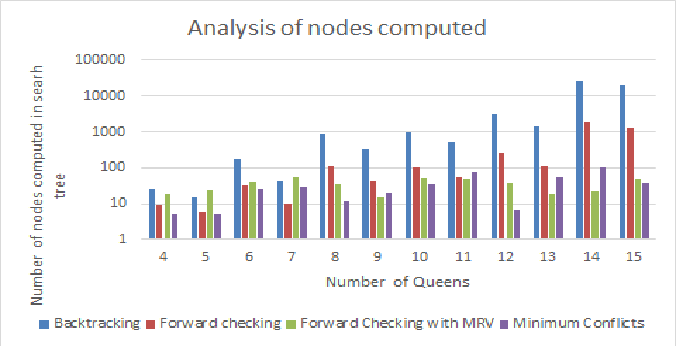
\includegraphics[scale=0.51]{XLS_nodesComputed.png}
\caption{Analysis of nodes computed}
\label{Figure10}
\end{figure}


\begin{figure}
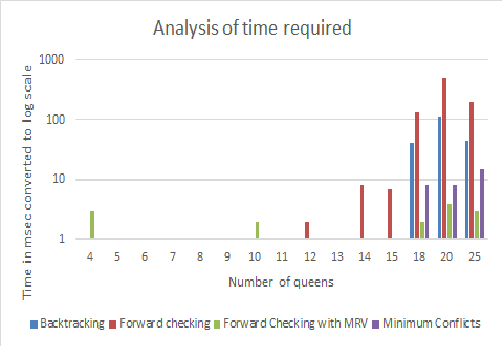
\includegraphics[scale=0.61]{XLS_time.png}
\caption{Analysis of time required}
\label{Figure11}
\end{figure}


\section{Conclusion}
Based on my experimental analysis, minimum conflicts approach proves to be the best approach for solving N-Queens problem as compared to backtracking, forward checking, and forward checking with MRV. It is better, both in terms of number nodes computed, i.e, equal to the number of steps in minimum conflicts as well as the time required to get to the solution. One by one computing the values for the variables recursively in the search tree does not help in the case of N-Queens. In fact, such techniques just need more time and huge memory for computing the solutions.

\begin{thebibliography}{11}

\bibitem{NQueensApplications}
Information on the n Queens problem
\\http://theory.cs.uvic.ca/amof/e\_queeI.htm

\bibitem{NqueensProblemGoogle}
The N-queens Problem
\\https://developers.google.com/optimization/puzzles/queens\#overview

\bibitem{experimentalComparisonPaper}
Kuruvilla Mathew and Mujahid Tabassum, Experimental Comparison of Uninformed and Heuristic AI Algorithms for N Puzzle and 8 Queen Puzzle Solution 

\bibitem{N-Queens genetic actual started}
 K. D. Crawford, “Solving the N-Queens Problem Using GA”.\\  In  Proceedings  ACM/SIGAPP  Symposium  on Applied  Computing,  Kansas  City,  1992,  pages  1039- 1047. 
 
\bibitem{Example paper of genetic N queens}
 Marko Božiković, Marin Golub, Leo Budin, Solving n-Queen problem using  global parallel genetic algorithm

\bibitem{Artificial Intelligence book}
Book by Stuart J. Russell and Peter Norvig, Artificial Intelligence, A Modern Approach, Third Edition 

\bibitem{exampleimagesBTandFC}
Constraint Propagation
\\http://ktiml.mff.cuni.cz/~bartak/constraints/propagation.html\#compare


\end{thebibliography}

% that's all folks
\end{document}


